\chapter{Background} \label{Background}

Functional programming uses immutable values and mathematical functions, also known as pure functions, to build programs. Similarly to imperative procedures, pure functions take parameters as input and compute some output. Unlike imperative procedures, however, pure functions are \textbf{only} allowed to transform their inputs to outputs and cannot have any other observable effects. Given the same inputs, a pure function must always evaluate to the same outputs. Abstraction and reuse, similarly to in imperative programs, is achieved by composing functions by passing the output of the previous function to the next function's input. The entire program can be seen as a large function composition of all functions used in the program.

A major difference between imperative and functional programming is in how one can reason about procedure or function compositions. Any expression in functional programming can always be \emph{substituted} with its value without changing the meaning of the program. The same does not apply in imperative programming. There is an implicit temporal coupling between imperative statements, since a statement may depend on the state set by previous statements. Because of this, reordering procedure calls or substituting any procedure call with its return value might change the meaning of the program.~\cite[Chapter~1]{sicp}

A program is considered to be \emph{referentially transparent} if it is possible to substitute an arbitrary expression in the program with its corresponding value without changing the meaning of the program in any way. Referentially transparent programs are easier to understand since they enable \emph{equational reasoning}, also known as \emph{local reasoning}. When composing pure functions, one does not have to understand their implementation, because the only effect the function is allowed to have is to return a result. A developer can only focus on the \emph{function's signature} and its specification, that is, what are the inputs and what is the output. Compilers can also take advantage of referential transparency by safely reordering expressions, evaluating expressions at compile time, memoizing results or by completely skipping the evaluation of expressions that are not required.

Referential transparency is one of the biggest differentiating factors between functional and imperative programming. Abandoning referential transparency has wide-reaching implications. In practice, it makes it much more difficult to refactor and develop programs. Developers are required to be more disciplined and to have wider knowledge of the whole program in order to not unintentionally cause defects. This is particularly evident when programming in the presence of concurrency, where side-effects can lead to race conditions and hard-to-reproduce errors.~\cite[Chapter~3]{sicp}

This chapter introduces first what effects are and discusses certain common effect types in more detail. Then it presents what concurrency is, how it can be achieved and what kind of problems it causes. Structured concurrency, a concept for defining semantics on how concurrent workflows interact, is also introduced. Lastly, the history and features relevant to managing side effects of the Scala programming language are introduced.



\section{Effects} \label{effects}
Constructing programs only by composing pure expressions without any notion of impurity is quite limiting, to say the least. To be useful in practice, programs depend on effects. An expression is said to have an effect, if its sole purpose is not to evaluate to a value or if its evaluation requires interacting with the outside world. For example, printing to the console, accessing the system clock or doing IO are all examples of effects. There is no unambiguous and exact definition of what an effect is, although the concept has been given, somewhat differing, characterizations by many.

\textcite{den-lang-specs} suggest that \textquote{A complete program is thought of as an agent that interacts with the outside world, e.g., a file system, and that affects global resources, e.g., the store [mutable memory]}. They continue by stating that every phrase in a program could be classified to either a value or an effect. A value is a referentially transparent expression, while an effect is an interaction with resources allocated for the program. When an effect is encountered, the control is transferred to a \textquote{central authority}. The central authority manages the use of all resources the program has access to. They continue to describe the interaction between an effect and the central authority:
\begin{displayquote}
An effect is most easily understood as an interaction between a sub-expression
and a central authority that administers the global resources of a program. (..) Given an administrator, an effect can be viewed as a message to the central authority plus enough information to resume the suspended calculation.
\end{displayquote}

\textcite{imperative-fp} as well as \textcite{do-be-do-be-do} see the distinction between expressions and effects as \emph{being} vs. \emph{doing}. This observation is quite interesting since it brings up the concept of computations as values. Certain approaches deliberately differentiate computations from values, while some deliberately unify them. It is later discussed how separation of effects from values applies to monadic effects and algebraic effects with handlers, together with the concept of a central authority presented earlier.

Different effects could be categorized as \emph{internal} or \emph{external}. Unlike internal effects, external effects can be observed from the outside. In the context of a whole program, the only external effect is IO, while other effects are internal. In the context of a function, matters are more complicated since effects such as mutable state, raising exceptions, and concurrency can be both internal or external, depending on the specific situation.


\subsection{Mutability} 
Mutability means that the program is able to change the state of the program, usually by mutating data stored in some memory location, and that it is possible to detect a state change by observing the changed value. Several control structures and language features require mutability. The destructive assignment operation found in almost every mainstream language is by definition mutation.~\cite[Chapter~3]{sicp} Looping constructs such as \inlinecode{for}- and \inlinecode{while} loops or iterators found in many standard libraries rely heavily on the notion of mutation. Also parts of some well known algorithms, like the swap operation in quicksort, can be expressed trivially as mutation.

In practice, almost all programs have some state that determines how the program reacts to input. Real-world examples of state include the location of characters in a game, registered users in an application and cursor position in the buffer when reading bytes from a socket. In the presence of concurrency, when parallel computations are expected to interact with each other, mutability in one form or another is needed to indicate if a computation is still on-going, completed or has encountered an error.


\subsection{Exceptions} \label{effect-types:exceptions}
Another very common effect is the ability to signal about exceptional conditions where the program is unable to compute a result or execute a command. This signaling is achieved by raising an error or exception. An exception could contain information about the condition that caused it, for example malformatted input, and that could possibly be later used when \emph{handling} or recovering from the exception. There are several common reasons why exceptions arise. They usually fall into two categories: technical or logical.~\cite{imprecise-exceptions}

Logical exceptions are usually caused by failing to meet some preconditions regarding the program's state or a function's parameters. A function may have assumptions about its inputs --- a string may need to be in a format that matches a schema in order to parse it successfully, or an integer may need to be positive and less than a certain threshold to represent a year. Sometimes inputs must be compatible with other inputs. An example of this is accessing an array by its index where the accessed index must be less than or equal to the size of the array, or attempting to access authorized content before proper authentication and authorization process.

Technical exceptions are usually related to IO, external events, the runtime environment, or the programming language itself. They can further be divided into synchronous and asynchronous exceptions. Peyton Jones describes synchronous exceptions as something that "arise as a direct result of some piece of code"~\cite{akward-squad}.  On the other hand, asynchronous exceptions are caused by external events and they cannot always be tied to the execution of a particular line of code. In some way, logical and synchronous exceptions are expected exceptions, and asynchronous exceptions are unexpected.

Many synchronous exceptions are related to IO. If attempting to interact with a file that does not exist or the current permissions are not sufficient, the result will likely be an exception of some sort. A significant source of exceptions is communicating over the network with a remote party. Everything from name resolution, routing, transport protocol or communication schema could go wrong. A remote component in a distributed system could be completely unavailable due to a network error or an internal error in that specific component. IO problems also arise when trying to perform an action before initialization, for example via a database connection, file descriptor or IO port.

Other synchronous exceptions may be caused by division by zero or a non-exhaustive pattern match. Probably the most well known synchronous exception is the infamous null reference error, where the program is trying to dereference a pointer that does not point to a valid memory location. In languages that support direct memory access, an attempt to access memory outside of the allowed memory range leads to a program or operating system level exception.~\cite{akward-squad}

Asynchronous exceptions usually originate from the runtime environment of the program, operating system, concurrency, or user interruption. Asynchronously raised exceptions are characterized by the fact that they could occur at an arbitrary point in time~\cite{async-exc}. An example of this is a situation where a thread interrupts the execution of another thread. The whole program could also be interrupted by a user (for example by pressing Ctrl+C) or the runtime, possibly due to a critical error in the program or operating system. Resource exhaustion is another common cause of asynchronous exceptions. Errors like stack overflow or out of memory can happen every time new memory is required from the stack or heap, thus those are categorized as asynchronous. Many environments also support dependencies to libraries that are loaded/linked  dynamically at run time. The programmer cannot always specify the exact time when dynamic loading should take place, and for this reason failing to load required dependencies could be considered an asynchronous exception.~\cite{akward-squad}

Exceptions can also encode another related and important concept, \emph{optionality}. Encoding optionality via exceptions is achieved by raising an exception that contains only a value of the unit type\footnote{A type whose cardinality is 1 (i.e., that has only one value) and thus does not contain any information.}, signaling that no result could be computed and there is no additional information about the exception. Optionality is an approriate choice instead of exceptions when the cause of the exception is trivial. Such cases include unsuccessfully querying a row from a database with specific id, searching an element from an array or trying to find a substring from a string.

Usually, the semantics of raising and handling an error are to interrupt the normal control flow of the program and transfer the execution to the closest appropriate \emph{exception handler}. An exception handler decides if and how to continue the execution, or whether to let the exception bubble up the layers of exception handlers. This "short-circuiting" semantics is a natural way to think and program in the presence of errors. However, the ability to raise errors from an arbitrary location can make it difficult to understand the meaning of the program and prove its correctness. It is a challenge to ensure that all exceptions that may be raised are handled appropriately. Lazy evaluation complicates things even further. The evaluation order in a lazily evaluated language may not be obvious to the programmer. This makes it harder to define clear semantics for exceptions.~\cite{imprecise-exceptions}

Effective and thorough exception handling is one of the most important practices in successful software engineering. Conversely, the inability to do so is one of the most significant factors that cause bugs and failures in software systems. A 2014 study by the University of Toronto studied multiple popular open source distributed software systems, such as Redis, Hadoop and Cassandra and found that a large portion (35\%) of catastrophical failures were caused by trivial mistakes in error handling code. Such mistakes include practices like omitting error handling code completely and writing a TODO-comment instead. In addition to failures, inadequate error handling may expose security vulnerabilities in the system.~\cite{simple-testing-failures}


\subsection{IO}
Programs need the ability to interact with the external world, i.e., with a user, other programs, or devices and sensors. IO is the medium to carry out these interactions. Like interaction in general, IO is often bidirectional --- the term IO is a shorthand for input and output. Input is the ability to observe changes and to receive information from other parties, output enables the program to cause changes in the environment and to dispatch information to others.

Many IO effects are about interacting with the user. Probably the most well-known and fundamental form of user interaction is to display text and graphics by changing pixels on the screen. Another common type of user interaction is via the console, which consists of printing characters to standard output and reading user input from standard input. The use of external devices such as playing sounds from speakers, recording sound from a microphone, or receiving user input from the keyboard, mouse, and touchscreen, is essential in user interaction.

In addition to user interaction, a program can also use devices for other purposes. For example, reading the time from the system clock, requesting the current temperature from a sensor, or setting a digital output to 1 or 0.

Often programs need the ability to store data that persists even when the program is restarted. This is achieved by using a device that allows reading from and writing to a non-volatile memory, such as a hard drive or memory card. Usually an operating system abstracts this persistent data store by providing a file system. However, many embedded devices still communicate directly with persistent memory devices.

The reason for a program to exist is to eventually have an effect on the surrounding world. As IO is the only way to achieve this, it fundamentally distinguishes IO from other effects. Where other effects might be useful for structuring computations and expressing computations in certain ways, IO is \emph{the reason} for programs to exist in the first place~\cite{akward-squad}. To put it the other way around, it would be impossible to detect if a program is running or not if it would not be interacting with its environment.



\section{Concurrency}
Computer programs should be able to run multiple workflows interleaved (concurrency) or at the same time (parallelism). Programs often have many simultaneous users, all of whom should be able to use the program independently of each other. Also, it is characteristic of IO that a large portion of time is spent waiting for a response, rather than calculating results with local computing resources, mainly CPUs. When several operations can be performed in parallel performance improves and the underlying hardware is utilized efficiently.


\subsection{Concurrency adds complexity}
Often workflows must interact with other concurrent workflows. A parent workflow might spawn multiple child workflows and split a task between them. In some situations, one might run several workflows in parallel and choose the result that is computed the fastest, discarding all other results. Concurrent workflows sometimes must use a shared resource, like mutable memory, file, or database connection.

At first glance, these interactions may seem not particularly problematic, but concurrency complicates programs significantly. By default the execution order of concurrent workflows is nondeterministic, because of how tasks are scheduled (usually by the operating system) to run on actual hardware. Many statements in a programming language are compiled to or interpreted as several CPU instructions, executed sequentially at different clock cycles. A canonical example of this is the increment operator (\inlinecode{++} or \inlinecode{+=}), that first reads a variable's value with one instruction and then sets it to a new value with another. If another parallel workflow is updating the same variable at the same time, it might see the value between the two instructions, even though that is rarely the desired behavior. These kind of situations are called \emph{race conditions}.

In order to prevent race conditions, explicit countermeasures are required. One way is to \emph{synchronize} access to shared resources. Usually this means that before a workflow can enter a section of the program or use a shared resource, it must acquire an exclusive \emph{lock}. This means that only one of the workflows has access to the resource at given point of time. Another way, applicable to shared memory, is to use atomic compare-and-swap operations~\cite{concurrent-queue-algorithms}, which enable to observe and update some data, succeeding only if the data was not modified by another workflow in between.

Locks and atomic references are examples of low-level tools for managing concurrency. Each tool comes with a set of trade-offs. When a workflow must acquire multiple locks, a possibility for \emph{deadlock} arises. Deadlock is a situation where concurrent workflows are blocked by each other and neither can continue until the other releases a lock they are holding. Atomic operations can fail, and the failure must be handled for example by retrying until the operation succeeds. Basic atomic operations usually cannot guarantee the atomicity of operations spanning over many atomic references.


\subsection{Concurrency primitives}
In practice concurrency can be implemented with many different constructs. The lowest-level construct commonly accessible to programming languages is a \textit{thread}. It is an OS level abstraction for concurrent execution. Each thread has its own stack, instruction pointer and CPU register values. All threads created by a single process share the same memory space, i.e. they are able to read from and write to the same shared memory blocks.

Threads are run on the actual hardware of the computer; a modern multi-core CPU can execute several workflows in parallel. The OS \textit{schedules} different threads for execution, and after a thread has been executing for a scheduled amount of time, the operating system interrupts the execution and switches the execution to a different thread. The operation where a CPU core switches the execution from one thread to another is called \textit{context switch}. Context switch requires that CPU registers and stack of the previous thread are saved, and respectively registers and stack of the new thread is loaded to the CPU.

% Threads
Traditionally a thread has been the concurrency primitive to turn to when some form of parallelism is required. Threads, however, are not a lightweight construct and they can exist only in limited numbers, usually in the thousands. Context switching between threads involves a significant amount of work, and thus causes performance overhead. Often a context switch defeats many optimizations in contemporary CPUs like caching, pipelining and speculative execution, which in turn amplifies the performance overhead. The issue manifests itself particularly in highly concurrent scenarios where computations are IO bound, which is usually the case in web and enterprise applications.

% Thread pools
A common way to constrain the total number of threads and increase their reuse is to collect multiple threads into a \emph{pool} of threads, where tasks could be submitted for execution instead of operating with individual threads. Once a task is submitted to a thread pool, it is queued and run once there are available threads. This way many concurrent workflows could be \emph{multiplexed} into a smaller number of physical threads. When fewer threads are created and reused by multiple concurrent workflows, the intent is to decrease the number of context switches in the hope of performance gains.

% Cooperative scheduling
Thread pools do not solve the problem that when a thread is waiting an IO operation or another thread to complete, the waiting thread is blocked. When a thread blocks, the OS puts it in a waiting state, meaning that its execution is not continued until the event it is waiting on is triggered. The ideal solution would be that no physical threads are blocked, and blocking is only semantic. This is not possible when threads are preemptively scheduled by the OS. A solution is to change the scheduling model from preemptive to \emph{cooperative}. Cooperative scheduling means that when a workflow is about to be blocked, it will register itself to be scheduled once all of its dependencies are met, and yield the control to other workflows. In this model no physical threads need to be blocked.

% Event loops
Cooperative scheduling is usually implemented by a runtime environment, programming language, or library, that runs on top of preemptively scheduled OS threads. Event loop is a common pattern for implementing cooperative scheduling, and it is used extensively in asynchronous IO or single-threaded environments like JavaScript. The idea is to have a queue that contains computations waiting to get executed, and the event loop picks up and executes tasks from the queue one at a time. Once a task is about the do a blocking operation, it registers a callback. The callback is invoked when the blocking operation completes, and it will add another task to the queue that represents the remaining of the workflow.

% Fibers
Another way to implement cooperative scheduling is \textit{fibers}. They are lightweight threads that are managed and scheduled in the application instead of OS. Each fiber contains a stack and possibly error handlers or thread-local variables, similar to a thread. Fibers require a scheduler that determines what fibers to execute on actual OS threads. The scheduler can multiplex many fibers to run on smaller number of physical threads. Fibers could exist in the hundreds of thousands or millions, and switching execution from one fiber to another is very cheap in comparison to a context switch between threads. The fiber scheduler can assign a fiber to execute on a specific CPU core, which will make it easier to reap benefits from CPU optimizations like caches.


\subsection{Structured concurrency}
When parent workflow spawns many child workflows, it is common that if one of the children encounters an error, the result cannot be computed at all and thus the results of other sibling workflows are not needed anymore. A similar situation can happen with racing workflows: when the first workflow successfully computes a result, the results of other workflows are no longer needed. In both of these situations it would be ideal to cancel the workflows whose results are not needed, to preserve compute resources and make sure that no concurrent workflows remain in execution. Traditional concurrency primitives, such as threads, do not offer this kind of control out of the box.

A solution to this is \textit{structured concurrency}~\cite{structured-concurrency, go-statement-considered-harmful}, which makes it possible to define clear semantics on if and how a child workflow could outlive its parent. The basic idea of structured concurrency is that there is a way to govern how child workflows are handled when the parent workflow completes (by succeeding or failing), or when there is an error encountered in any of the sibling workflows. For example, for a parent workflow that spawns child workflows one would like to define whether the children should be awaited, cancelled, or left orphaned when the parent completes or is cancelled before the children are finished.

Native support for structured concurrency in programming languages is still quite rare, but it has been added to programming languages at an accelerating pace. Kotlin added structured concurrency back in 2018~\cite{kotlin-sc}, Swift 5.5 in 2021~\cite{swift-sc} and Java 19 in 2022~\cite{java-sc}. The feature will probably find its way into more programming languages in the future.

It is difficult to write correct and concurrent programs. Knowledge of concurrency primitives and tools, such as different data structures and CPU instructions, and possible concurrency hazards are required. One has to be especially careful about race conditions, which are not always obvious. Ideally, concurrency could be implemented with high-level code, using operations that take into consideration possible concurrency issues, and deal with low-level details.



\section{Scala} \label{scala}
Scala~\cite{scala-lang} is a high level, statically typed, compiled, and garbage collected programming language, that is both functional and object-oriented. It is eagerly evaluated by default, but supports also lazy evaluation. The first release was in 2004 and the latest version is 3, which was released in 2021. Version 3 is exclusively used in this thesis. The initial and current lead designer of the language is Martin Odersky, a professor at the École polytechnique fédérale de Lausanne. Scala's roots are thus in academia, but its approach is pragmatic.

Scala is most commonly run on the \acronym{JVM}{Java Virtual Machine}, but also JavaScript and native code are supported compilation targets. When running on the JVM it is possible to use Java code directly from Scala. The Scala standard library even contains functions for converting Java data types to their Scala counterparts. This gives access to a huge number of Java libraries.

Scala aims to blend the \acronym{FP}{Functional programming} and \acronym{OOP}{Object-oriented programming} paradigms and as a result has features from both. Many OOP concepts like classes, objects, interfaces and subtype polymorphism are supported. In fact, every value in Scala is an object. Scala uses class-based objects with attributes and methods, and supports multiple inheritance. Scala supports generics with lower and upper subtype constraints as well as declaration-site variance. The language also includes many imperative constructs, like loops and mutable variables, that are commonly used in other OO-languages. Perhaps less common in OO-languages, in Scala everything is an expression, including control structures like \inlinecode{if/else}, \inlinecode{try/catch}, and loops. \refsource{scala:basics} demonstrates the basic syntax of Scala.

\begin{algorithm}

\begin{minted}{scala}
trait Foo // Define an interface
class Bar extends Foo // Define a class inheriting from Foo

// Define variables/constants
var mutableFoo: Foo = Bar() // Explicit type is Foo
val immutableBar    = Bar() // Inferred type is Bar
lazy val lazyPlus   = 1 + 1 // Computed lazily and cached

// Type argument here is Int
val genericType: List[Int] = List(1, 2, 3)

// Type parameters are declared between '[' and ']'
def genericMethod[A](a: A): A = a

// Type parameter constraints:
// 'A' must be supertype of 'Bar' and  'B' must be subtype of 'Foo'
def typeBounds[A >: Bar, B <: Foo](a: A): B = ???

// ??? is defined in the standard library. It can replace any
// expression; it's type is Nothing, the bottom type
def `???` : Nothing = throw new NotImplementedError

// => specifies 'by-name' calling convention:
// The parameter n is evaluated every time it is used (2 times here)
def byNameParameter(n: => Int) = n + n
\end{minted}

\caption{Basic syntax of Scala. \label{scala:basics}}
\end{algorithm}

Due to Scala's object-oriented nature, every object is part of a type hierarchy. On top of the hierarchy is \inlinecode{Any}, which is the supertype of all other types. Below \inlinecode{Any} is \inlinecode{Matchable}, which marks values suitable for pattern matching. \inlinecode{Matchable} has two subtypes: \inlinecode{AnyVal}, a supertype for all value types, and \inlinecode{AnyRef}, a supertype for all reference types. \inlinecode{Null} is a subtype of all reference types, except when \emph{explicit nulls} -feature is enabled and \inlinecode{Null} becomes a subtype of \inlinecode{Any}. Scala also has a bottom type \inlinecode{Nothing} that is a subtype of every type. No values of type \inlinecode{Nothing} can ever exist at runtime so the type reflects the absence of a value, for example in the case of infinite recursion or loop, or when the expression throws an exception. The diagram in Figure \ref{fig:scala-type-hierarchy} depicts the type hierarchy.

\begin{figure}
    \centering
    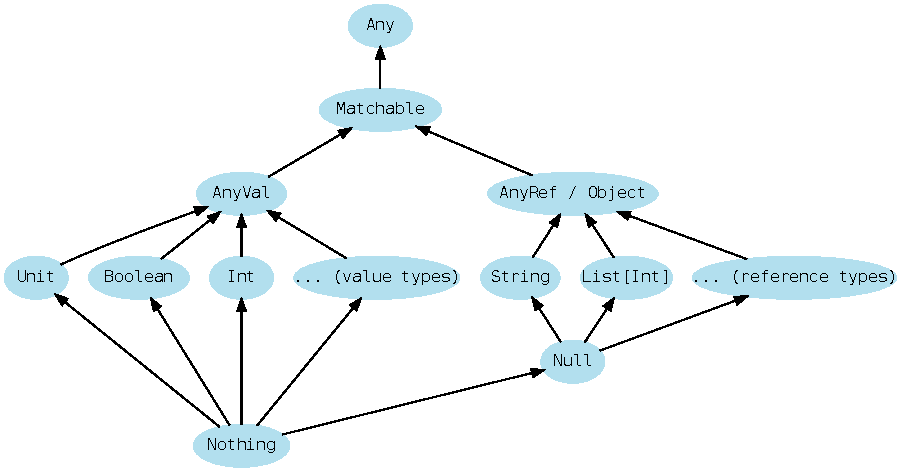
\includegraphics[width=\textwidth]{images/type-hierarchy}
    \caption{Scala 3 type hierarchy.}
    \label{fig:scala-type-hierarchy}
\end{figure}

Variance defines the rules on how the subtype relationships between parameterized types are dependent on the subtype relationship on the type on which it is parameterized. Variance has three variants: \emph{invariance}, \emph{covariance}, and \emph{contravariance}. Invariance means that subtyping relationships present in type parameters are not applied to the parameterized type at all. Covariance states that the subtype relationship of the parameterized type are in the same direction as a type parameter's subtype relationship. Contravariance means that the subtype relationship between parameterized types are the opposite way compared to the subtype relationships of the type parameter. When \inlinecode{Sub} is a subtype of \inlinecode{Super} and \inlinescala{F[_]} is any parameterized type, then
\begin{itemize}
    \item Under covariance, \inlinescala{F[Sub]} is a subtype of \inlinescala{F[Super]};
    \item Under contravariance, \inlinescala{F[Super]} is a subtype of \inlinescala{F[Sub]}; and
    \item Under invariance, \inlinescala{F[Sub]} and \inlinescala{F[Super]} have no subtyping relationship.
\end{itemize}

Covariance is applicable in parameterized types that contain, store, or produce values, in other words the type parameter is in covariant position. Contravariance is applicable in the opposite situation, where values of the type parameter are consumed, i.e. the type parameter appears in a function parameter list, and is said to be in contravariant position. Invariance is useful in situations where it does not make sense for the parameterized type to have inheritance based on type parameter, or when the parameterized type is a mutable, or the type parameter appears both in covariant and contravariant positions. A parametric type with multiple type parameters could declare each type parameter with different variance. For example functions in Scala are contravariant in their input type(s) and covariant in their result type.

An infamous example of a mutable covariant type is the primitive array type in Java and C\#.
These arrays must perform a runtime type check when adding elements to the array, and throw an exception if the type of the element is not compatible with the array, as demonstrated in \refsource{mutable-covariance}. To avoid these mandatory costs and checks, mutable collections in Scala are invariant. Immutable collections and containers, such as \inlinecode{Option} or \inlinecode{Either} are covariant in Scala.

\begin{algorithm}

\begin{minted}{java}
String[] a = new String[1];	
Object[] b = a; // String is a subtype of Object, so this is legal
b[0] = 1; // Runtime exception since cannot add Integer to String[]
\end{minted}

\caption{Covariance in mutable types, like Java primitive array, is problematic \label{mutable-covariance}}
\end{algorithm}

Programming languages differ in the way variance annotations are defined and used. Variance annotations in C\# and Scala are with the parameterized type. On the other hand, in Java one defines variance only when using a parameterized type. The former is called \emph{declaration-site} variance, demonstrated in \refsource{declaration-site-variance} and the latter is called \emph{use-site} variance, demonstrated in \refsource{use-site-variance}. Approaches deviating from these exist, for example TypeScript tries to infer variance, but it has optional declaration-site annotations from version 4.7 onwards. Kotlin has declaration-site variance by default but it emulates some parts of use-site variance with type projections.

\begin{algorithm}

\begin{minted}{scala}
class Invariant[A]      // Invariance is the default
class Covariant[+A]     // Covariance denoted with +
class Contravariant[-A] // Contravariance denoted with -
\end{minted}

\caption{Scala uses declaration-site variance, where the variance of a parameterized type is denoted in its type definition  \label{declaration-site-variance}}
\end{algorithm}

\begin{algorithm}

\begin{minted}{java}
interface Supertype {}
interface Subtype extends Supertype {}

void invariant(List<Supertype> list) {
    /* Get and set list values */
}
void covariant(List<? extends Supertype> list) {
    /* Only get list values */
}
void contravariant(List<? super Subtype> list) {
    /* Only set list values */
}
\end{minted}

\caption{Java has use-site variance, where the desired variance is declared when using the parameterized type \label{use-site-variance}}
\end{algorithm}

Invariance is the default in Scala and it does not require an explicit annotation. Covariance is declared with a \inlinecode{+} sign before each type parameter. Since contravariance could be seen as the opposite of covariance, it is denoted with a \inlinecode{-} sign.

Many features and principles from functional programming are not only available, but also encouraged in Scala. Pattern matching, first-class functions (\refsource{scala:lambdas}), and tail recursion are all supported and heavily utilized in idiomatic Scala programs. Immutable variables, collections and data-structures are the default way of writing Scala, even though mutable counterparts are also available. Functional data modeling is achieved with the use algebraic data types built into the language. Even though Scala embraces functional programming and imperative code is generally discouraged, introducing arbitrary side effects is possible.

\begin{algorithm}
\begin{minted}{scala}
val ns = List(1, 2, 3)

val mapped1 = ns.map(n => n + 1)
val mapped2 = ns.map(_ + 1) // Same as above in shorter form

val sum1 = ns.foldLeft(0)((x, y) => x + y)
val sum2 = ns.foldLeft(0)(_ + _) // Same as above in shorter form
\end{minted}

\caption{Long and short form of anonymous functions in Scala. \label{scala:lambdas}}
\end{algorithm}

In addition to ordinary functions, Scala has a specific function type called \\\inlinecode{PartialFunction} for representing functions that are not defined for all values of their input types. It is a subtype of the (normal) function type, to which it adds the method \inlinecode{isDefinedAt}, which determines if the function is defined for a given value. \refsource{scala:partial-function} shows how to define and use partial functions.

\begin{algorithm}
\begin{minted}{scala}
val someEvensMultipliedByTen: PartialFunction[Option[Int], Int] = {
  case Some(n) if n % 2 == 0 => n * 10
}

val opts  = List(None, Some(2), None, Some(3), Some(4))
val somes = opts.collect(someEvensMultiplied) // List(20, 40)
\end{minted}

\caption{Partial functions in Scala. \label{scala:partial-function}}
\end{algorithm}

Some functional languages, such as Haskell, have a special syntax for monadic computations. Scala also provides this syntactic sugar in a form of \inlinecode{for} comprehensions, demonstrated in \refsource{monad:for-syntax}. For comprehension is compatible with any data type that has \inlinecode{map} and \inlinecode{flatMap} methods defnied, such as \inlinecode{Option}, \inlinecode{Either}, and \inlinecode{ZIO} (Chapter \ref{zio}). These required methods can be added to any type by using extension methods.

Extension methods, which allow adding methods to a class separately from its definition, are one of Scala's more advanced features. Other state-of-the-art features of Scala include operator overloading and infix operator- and method syntax, higher kinded and dependent types, type lambdas, as well as powerful meta programming capabilities. Scala 3 introduced more cutting edge features, such as automatic type class derivation and union and intersections types.

Probably the most distinguishing feature in Scala is its system of implicits and other contextual abstractions arising from that. A function can mark some of its parameters as implicit and the compiler will try to figure out that parameter from the enclosing scope by its type without the programmer explicitly passing an argument for that parameter. Originally implicit parameters were introduced to achieve similar behavior as Haskell's type classes. Implicits can, however, also be used for other purposes, such as implicit conversions, context propagation, extension methods, and proving subtyping relationships between generic type parameters at compile-time.~\cite{tc-as-objects}

Syntactically to use implicits, a function can mark some of its parameters as implicit with the keyword \inlinecode{using}. When the function is called, the compiler tries to find a value marked as implicit, with the keyword \inlinecode{given}, from the enclosing scope. If all requested values are found, they are automatically applied as arguments. If any of the implicit parameters is not found, compilation error is reported. \refsource{scala:implicits} shows the function \inlinecode{summon} that searches for an implicit value by type, demonstrating the definition and use of implicit parameters.

\begin{algorithm}
\begin{minted}{scala}
case class Person(age: Int, name: String)

// Define type class
trait Show[A]:
  extension (a: A) def show: String

// Define type class instance
given Show[Person] with
  extension (a: Person)
    def show: String = s"${a.name} is ${a.age} years old"

// Use the type class
def showAll[A: Show](as: List[A]): List[String] =
  as.map(a => a.show)
\end{minted}

\caption{Implicits could be used to encode type classes \label{scala:typeclasses}}
\end{algorithm}

Another advanced feature utilizing implicit resolution is the ability of the Scala compiler to prove type equality or subtype relationships. The class \inlinescala{=:=[From, To]} is for type equality and \inlinescala{<:<[From, To]} for subtype relationship. Both classes extend a function \inlinescala{From => To}, and can be used to transform types. Types with two type parameters could be used as infix in Scala, for example type equality could be written \inlinescala{A =:= B}. When requesting an implicit parameter of either of the types above, Scala compiler synthesizes an instance if the type relationship holds, otherwise reports a compilation error. The act of proving type relationships is said to be \emph{witnessing}, and a common practice is to name the implicit parameter as \emph{evidence}. The feature is useful, for example, when defining functions that make sense only for specific types, as demonstrated in \refsource{scala:witness}, where only nested \inlinecode{Maybe} types could be flattened.

\begin{algorithm}
\begin{minted}{scala}
enum Maybe[+A]:
  case Just(a: A)
  case Nothing

  def flatten[B](using evidence: A <:< Maybe[B]): Maybe[B] =
    this match
      case Just(a) => evidence(a)
      case Nothing => Nothing

Maybe.Just(Maybe.Just(1)).flatten // Compiles
Maybe.Just(1).flatten // Error: Cannot prove that Int <:< Maybe[B]
\end{minted}

\caption{Scala compiler can prove (witness) a subtype relationship by providing implicit evidence. \label{scala:witness}}
\end{algorithm}

Another thing that sets Scala 2 and 3 apart is the introduction of intersection and union types in Scala 3. Intersection types are denoted with the \inlinecode{&} symbol and union types with \inlinecode{|}. Intersection \inlinescala{A & B} means that the resulting type has properties of both \inlinecode{A} \textbf{and} \inlinecode{B}. Union is the dual of intersection, and the resulting type of \inlinescala{A | B} is either \inlinecode{A} \textbf{or} \inlinecode{B}.

Intersection types are commutative, idempotent, and have \inlinecode{Any} as the identity element. Commutativity means that the order of types included in the intersection does not matter --- Scala considers permutations equal. Idempotency means that type intersectioned with itself is equal to the type itself. \inlinecode{Any} as the identity element means that the intersection of any type \inlinecode{A} with \inlinecode{Any} is equal to \inlinecode{A}, since all types themselves are subtypes of \inlinecode{Any}. Expressed as code, laws of intersection types can be proved with the Scala compiler:
\begin{itemize}
    \item Commutativity: \inlinescala{summon[(A & B) =:= (B & A)]}
    \item Idempotency: \inlinescala{summon[A =:= (A & A)]}
    \item Identity: \inlinescala{summon[A =:= (A & Any)]}
\end{itemize}

Like intersection types, also union types are commutative, idempotent, and obey the identity laws. The identity element is \inlinecode{Nothing}: the union of any type \inlinecode{A} with \inlinecode{Nothing} is equal to \inlinecode{A}, since there are no values of type \inlinecode{Nothing}. Again expressed as code, the laws of union types proved by the Scala compiler are:
\begin{itemize}
    \item Commutativity: \inlinescala{summon[(A | B) =:= (B | A)]}
    then\item Idempotency: \inlinescala{summon[A =:= (A | A)]}
    \item Identity: \inlinescala{summon[A =:= (A | Nothing)]}
\end{itemize}
